\documentclass[12pt]{report}
\usepackage[nottoc]{tocbibind}
\usepackage{tocloft}
\usepackage{hyperref}
\usepackage{titlesec}
\usepackage{enumitem}
\usepackage{graphicx}
\usepackage{caption}
\usepackage{float}
\usepackage{geometry}
\usepackage{animate}
\usepackage{listings}
\usepackage[T1]{fontenc}
\usepackage[italian]{babel}
\usepackage{setspace}

\renewcommand{\contentsname}{Indice}
\renewcommand{\figurename}{Figura}
\renewcommand{\tablename}{Tabella}
\counterwithout{figure}{chapter}
\counterwithout{table}{chapter}
% Copyright 2017 Sergei Tikhomirov, MIT License
% https://github.com/s-tikhomirov/solidity-latex-highlighting/

\usepackage{listings, xcolor}

\definecolor{verylightgray}{rgb}{.97,.97,.97}

\lstdefinelanguage{Solidity}{
	keywords=[1]{anonymous, assembly, assert, balance, break, call, callcode, case, catch, class, constant, continue, constructor, contract, debugger, default, delegatecall, delete, do, else, emit, event, experimental, export, external, false, finally, for, function, gas, if, implements, import, in, indexed, instanceof, interface, internal, is, length, library, log0, log1, log2, log3, log4, memory, modifier, new, payable, pragma, private, protected, public, pure, push, require, return, returns, revert, selfdestruct, send, solidity, storage, struct, suicide, super, switch, then, this, throw, transfer, true, try, typeof, using, value, view, while, with, addmod, ecrecover, keccak256, mulmod, ripemd160, sha256, sha3}, % generic keywords including crypto operations
	keywordstyle=[1]\color{blue}\bfseries,
	keywords=[2]{address, bool, byte, bytes, bytes1, bytes2, bytes3, bytes4, bytes5, bytes6, bytes7, bytes8, bytes9, bytes10, bytes11, bytes12, bytes13, bytes14, bytes15, bytes16, bytes17, bytes18, bytes19, bytes20, bytes21, bytes22, bytes23, bytes24, bytes25, bytes26, bytes27, bytes28, bytes29, bytes30, bytes31, bytes32, enum, int, int8, int16, int24, int32, int40, int48, int56, int64, int72, int80, int88, int96, int104, int112, int120, int128, int136, int144, int152, int160, int168, int176, int184, int192, int200, int208, int216, int224, int232, int240, int248, int256, mapping, string, uint, uint8, uint16, uint24, uint32, uint40, uint48, uint56, uint64, uint72, uint80, uint88, uint96, uint104, uint112, uint120, uint128, uint136, uint144, uint152, uint160, uint168, uint176, uint184, uint192, uint200, uint208, uint216, uint224, uint232, uint240, uint248, uint256, var, void, ether, finney, szabo, wei, days, hours, minutes, seconds, weeks, years},	% types; money and time units
	keywordstyle=[2]\color{teal}\bfseries,
	keywords=[3]{block, blockhash, coinbase, difficulty, gaslimit, number, timestamp, msg, data, gas, sender, sig, value, now, tx, gasprice, origin},	% environment variables
	keywordstyle=[3]\color{violet}\bfseries,
	identifierstyle=\color{black},
	sensitive=true,
	comment=[l]{//},
	morecomment=[s]{/*}{*/},
	commentstyle=\color{gray}\ttfamily,
	stringstyle=\color{red}\ttfamily,
	morestring=[b]',
	morestring=[b]"
}

\lstset{
	language=Solidity,
	backgroundcolor=\color{verylightgray},
	extendedchars=true,
	basicstyle=\footnotesize\ttfamily,
	showstringspaces=false,
	showspaces=false,
	numbers=left,
	numberstyle=\footnotesize,
	numbersep=9pt,
	tabsize=2,
	breaklines=true,
	showtabs=false,
	captionpos=b
}

\usepackage{color}
\definecolor{lightgray}{rgb}{.9,.9,.9}
\definecolor{darkgray}{rgb}{.4,.4,.4}
\definecolor{purple}{rgb}{0.65, 0.12, 0.82}
\lstdefinelanguage{JavaScript}{
  keywords={break, case, catch, const, continue, debugger, default, delete, do, else, false, finally, for, function, if, in, instanceof, new, null, require, return, switch, this, throw, true, try, typeof, var, void, while, with},
  morecomment=[l]{//},
  morecomment=[s]{/*}{*/},
  morestring=[b]',
  morestring=[b]",
  ndkeywords={class, export, boolean, throw, implements, import, this},
  keywordstyle=\color{blue}\bfseries,
  ndkeywordstyle=\color{darkgray}\bfseries,
  identifierstyle=\color{black},
  commentstyle=\color{purple}\ttfamily,
  stringstyle=\color{red}\ttfamily,
  sensitive=true
}

\lstset{
   language=JavaScript,
   backgroundcolor=\color{lightgray},
   extendedchars=true,
   basicstyle=\footnotesize\ttfamily,
   showstringspaces=false,
   showspaces=false,
   numbers=left,
   numberstyle=\footnotesize,
   numbersep=9pt,
   tabsize=2,
   breaklines=true,
   showtabs=false,
   captionpos=b
}
\usepackage{listings}
\usepackage{xcolor}

\lstdefinelanguage{JSON}{
    string=[s]{"}{"},
    comment=[l]{:\ "},
    morecomment=[l]{:"},
}

\setlength{\cftbeforetoctitleskip}{-1cm}

\titleformat{\chapter}[display]
{\normalfont\bfseries\filcenter}
{Capitolo\ \thechapter}
{0pt}
{\Huge}

\titlespacing{\chapter}{0pt}{-20pt}{40pt}

\newenvironment{firstpagetableofcontents}
{\begin{center}\bfseries\end{center}\begin{center}\filcenter}
{\end{center}\clearpage}

\setcounter{tocdepth}{1}

\begin{document}

\thispagestyle{empty}
\begin{figure}[t]
    \vspace*{-0.5in}
    \centering
    
\includegraphics[width=1\textwidth]{tesiSCIENZE_TECNOLOGIE.jpg}
    \label{fig:titolo}
\end{figure}

\begin{center}
    \vspace*{-0.5in}\rule[1mm]{10cm}{0.2mm}
\end{center}

\begin{center}
    \large \bf{Corso di Laurea triennale in Informatica}
\end{center}

\vspace*{1.1in}
\begin{center}
    \linespread{1}\LARGE\bf{Il ruolo degli NFT nella protezione dei beni}
\end{center}

\begin{center}
    \vspace*{1.1in}
    \begin{tabular}{@{}l@{\hspace{1.5in}}l@{}}
        \large Relatore: & \large Candidato: \\
        \\
        \large Dott. Andrea Visconti & \large Daniele Reccagni, mat. 975771
    \end{tabular}
\end{center}

\vspace*{1.1in}
\begin{center}
    Anno accademico 2022/2023
\end{center}

\onehalfspacing

\newpage
\begin{firstpagetableofcontents}
\tableofcontents
\end{firstpagetableofcontents}

\chapter{Introduzione}
\noindent
La nascita e l'evoluzione del Web 3.0 stanno portando il controllo e la proprietà delle informazioni in transito su Internet nelle mani di chi effettivamente lo utilizza: l'approccio decentralizzato di gestione dei dati sta creando un sistema più equo e autonomo per gli utenti di Internet, rimuovendo gradualmente il necessario controllo esterno delle grandi aziende caratteristico dell'approccio centralizzato del Web 2.0.\newline
Termini come criptovalute, blockchain, finanza decentralizzata, token, NFT, metaverso e app decentralizzate sono concetti oramai diffusi, consolidati e ben noti ai più, e ci stiamo rendendo conto di quanto questi strumenti, se utilizzati in maniera intelligente, siano veramente molto potenti e possano dare una grande mano nell'evoluzione della società contemporanea.\newline\newline
La domanda che sorge quasi spontanea a questo punto è la seguente: è possibile utilizzare le entità sopra citate, o almeno alcune tra di esse, per risolvere problemi noti in modo semplice, veloce, economico e affidabile? La risposta è un convinto "sì" e la tecnologia può venire in nostro aiuto.\newline
In questo lavoro di tesi, infatti, l'obiettivo è stato di progettare e realizzare una soluzione concreta a uno di questi problemi sfruttando le tecniche crittografiche apprese durante il mio percorso di studi. Più precisamente, abbiamo ideato un sistema per garantire protezione ad un qualsiasi bene materiale, come ad esempio una scultura, una casa, una giacca di lusso o una bottiglia di un liquore pregiato.\newpage
\noindent
Cosa significa "garantire protezione" ad uno di questi oggetti? Immaginiamo una generica operazione di vendita tra un venditore ed un acquirente. Il nostro obiettivo è assicurare che in questo processo siano rispettate tre proprietà fondamentali:
\begin{itemize}[topsep=5pt, itemsep=0pt]
    \item Il venditore e l'acquirente siano realmente chi dicono di essere e non dei truffatori;
    \item Il venditore possegga veramente il bene che sta provando a vendere all'acquirente;
    \item Il bene venduto dal venditore all'acquirente sia autentico e non un falso.
\end{itemize}
Se ci pensiamo bene, queste sono proprio le garanzie che dà un notaio durante un atto di vendita. Ebbene, l'obiettivo è quindi di automatizzare il lavoro di un notaio utilizzando alcuni dei potenti strumenti del Web 3.0.\newline\newline
Si noti che, dal momento che il Web 3.0 è in costante crescita, alcune delle scelte/tecnologie descritte in questa tesi potrebbero risultare "superate" a stretto giro a causa delle continue evoluzioni tecnologiche.

\chapter{Concetti preliminari}
\noindent
Elenchiamo e analizziamo ora i più importanti strumenti che sono stati utilizzati durante la creazione del sistema di protezione, scendendo nei dettagli delle loro caratteristiche e del loro funzionamento.

\section{Funzioni hash}
Le funzioni hash sono delle funzioni crittografiche facilmente computabili che ricevono in input una stringa di dimensione qualsiasi e restituiscono in output una stringa di dimensione fissa.
Esse posseggono tre proprietà principali:
\begin{itemize}[topsep=5pt, itemsep=0pt]
    \item \textbf{Collision-free}\newline
    Non si è in grado di trovare \(X\) e \(Y\) tali che \(H(X) = H(Y)\) e \(X \neq Y\). In realtà queste collisioni esistono, ma dei regular users non sono in grado di trovarle.\newline
    Grazie a questa proprietà, possiamo assumere \(H(X) = H(Y)\) --> \(X = Y\) e, di conseguenza, possiamo salvare solo \(H(X)\) e \(H(Y)\) che, oltre ad occupare molto meno spazio, permettono di comparare dati usando molti meno bit rispetto ai dati in chiaro.
    \begin{figure}[H]
        \centering
        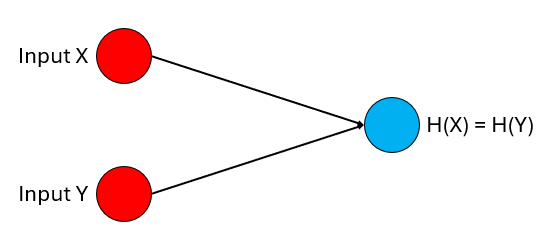
\includegraphics[width=0.6\textwidth]{Collision-free.PNG}
        \captionsetup{justification=centering}
        \caption{Proprietà collision-free \cite{Uno}}
        \label{fig:collisionfree}
    \end{figure}
    \item \textbf{Preimage resistant}\newline
    Le funzioni hash sono one-way function: dato \(H(X)\) è computazionalmente impossibile riuscire a risalire ad \(X\). Grazie a questa proprietà, l'unico modo per trovare \(X\) sarebbe un attacco bruteforce.
    \begin{figure}[H]
        \centering
        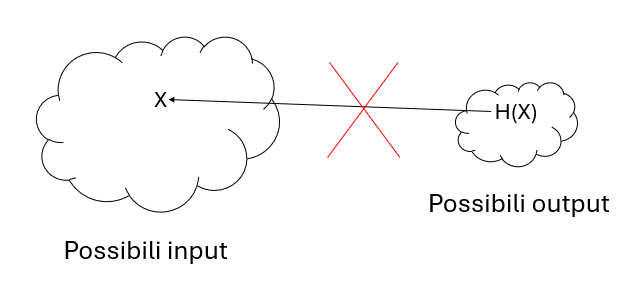
\includegraphics[width=0.6\textwidth]{Preimage resistant.PNG}
        \captionsetup{justification=centering}
        \caption{Proprietà preimage resistant \cite{Uno}}
        \label{fig:preimageresistant}
    \end{figure}
    \item \textbf{Second preimage resistant}\newline
    Conoscendo \(X\), \(H(X)\) e \(H(Y)\) non si è in grado di risalire ad \(Y\) tale che \(H(X) = H(Y)\) e \(X \neq Y\).
    \begin{figure}[H]
        \centering
        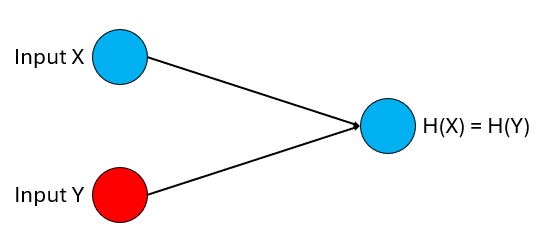
\includegraphics[width=0.6\textwidth]{Second preimage resistant.PNG}
        \captionsetup{justification=centering}
        \caption{Proprietà second preimage resistant \cite{Uno}}
        \label{fig:secondpreimageresistant}
    \end{figure}
\end{itemize}
Queste particolari funzioni sono usate, ad esempio, per provare l'integrità dei dati (confrontando l'hash dei dati in momenti diversi) o in ambito blockchain per mezzo di hash pointers. Proprio quest'ultimo è l'utilizzo sul quale ci concentreremo. \cite{Uno}\newline

\section{Hash pointer}
Un hash pointer è un evoluzione del concetto di puntatore classico.\newline
Se i puntatori normali memorizzano unicamente l'indirizzo di memoria dei dati a cui fanno riferimento e permettono di accedere facilmente ad essi, un hash pointer memorizza anche l'hash crittografico dei dati permettendo di verificare anche la loro integrità. Utilizzando questi hash pointers è possibile ottenere importantissimi concetti e strutture dati come le blockchain e gli alberi di Merkle. \cite{Due}\newline
\begin{figure}[H]
    \centering
    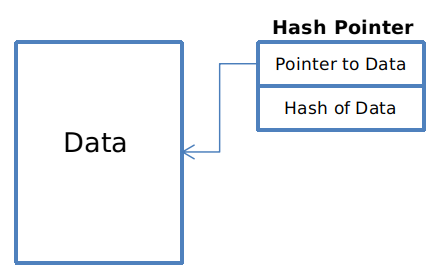
\includegraphics[width=0.6\textwidth]{Hash pointer.png}
    \captionsetup{justification=centering}
    \caption{Hash pointer \cite{Tre}}
    \label{fig:hashpointer}
\end{figure}

\section{Blockchain}
Una blockchain è un enorme registro globale distribuito su cui vengono salvati i dati di una serie di operazioni: le transazioni. Essa prende il nome dal modo in cui memorizza questi dati, ossia creando una catena di blocchi.\newline
Un blocco è un insieme di dati di transazione che ha raggiunto una certa dimensione considerevole. Quando questo avviene, tutte le transazioni a cui fa riferimento vengono convalidate e quindi archiviate in modo permanente all'interno della blockchain.\newline
I blocchi appena citati sono concatenati tra di loro formando il cosiddetto libro mastro immutabile. \cite{Quattro}
\subsection{Layers}
Esistono diversi livelli di blockchain, ognuno dei quali definisce delle caratteristiche importanti della chain stessa:
\begin{itemize}[topsep=5pt, itemsep=0pt]
    \item \textbf{Blockchain di livello 1}\newline
    Le blockchain di livello 1 sono le principali: eseguono e convalidano le transazioni da sole, senza assistenza, e hanno le proprie criptovalute associate.\newline
    Alcuni esempi di queste blockchain sono Ethereum, Solana e Avalanche.
    \item \textbf{Blockchain di livello 2}\newline
    Le blockchain di livello 2 sono utili per risolvere i problemi di scalabilità delle blockchain di livello 1. Esse elaborano le transazioni internamente e memorizzano solo un riepilogo delle azioni svolte sulla chain di livello 1.\newline
    Grazie a questa proprietà, le richieste alla blockchain principale sono ridotte di molto, migliorando la scalabilità e abbassando i costi dei gas fees, delle "tasse" da pagare per poter utilizzare la blockchain.\newline
    Optimism e Arbitrum sono degli esempi di questo tipo di blockchain.
    \item \textbf{Blockchain di livello 3}\newline
    Le blockchain di livello 3 aggiungono ulteriore scalabilità e interoperabilità tra diverse blockchain. Esse sono particolarmente utili per eseguire applicazioni decentralizzate.\newline
    Alcuni esempi sono Polkadot e Cosmos.
    \item \textbf{Sidechain}\newline
    Le sidechain sono molto simili alle blockchain di livello 2: sono anche'esse blockchain separate e collegate ad una chain di livello 1, ma sono molto più indipendenti e spesso hanno una criptovaluta personale.\newline
    Un classico esempio di sidechain è Polygon, una sidechain di Ethereum: gli utenti ottengono un'esperienza simile all'utilizzo di Ethereum, ma con gas fees più bassi e tempi di transazione più rapidi (vedi la \hyperref[sec:polygon]{Sezione 3.3}). \cite{Quattro}\newpage
\end{itemize}
\subsection{Meccanismi di consenso}
Un'altra caratteristica importante delle blockchain riguarda i meccanismi di consenso, cioè il modo in cui le transazioni vengono convalidate, ossia registrate in modo permanente nella blockchain.
Esistono due meccanismi principali:
\begin{itemize}[topsep=5pt, itemsep=0pt]
    \item \textbf{Proof-of-Stake}\newline
    Le blockchain che utilizzano il metodo Proof-of-Stake verificano le transazioni usando delle persone dette validators.\newline
    Quando un nuovo blocco di transazioni deve essere aggiunto alla blockchain, viene selezionato un validator in modo casuale. Egli creerà concretamente il blocco di transazioni e lo porrà in esame ad un comitato di altri validators, che voteranno se quel blocco è valido e quindi può essere memorizzato nella chain.\newline
    Le blockchain Proof-of-Stake sono molto più veloci, meno costose e più rispettose dell'ambiente rispetto a quelle Proof-of-Work, ma sono meno sicure.\newline
    Alcuni esempi sono Ethereum (post-Merge) e Polygon.
    \item \textbf{Proof-of-Work}\newline
    Le blockchain che utilizzano il metodo Proof-of-Work verificano le transazioni usando delle persone dette miners.\newline
    Quando un nuovo blocco di transazioni deve essere aggiunto alla blockchain, un gruppo di miners concorrerà per trovare un determinato numero, detto nonce, tale per cui una funzione di hash applicata sul blocco di transazioni e sul numero restituisca un altro numero con una certa quantità di zeri in testa.\newline
    Ogni qualvolta un miner comunichi pubblicamente di aver trovato il nonce corretto affinché si verifichi la condizione di cui sopra, gli altri miners si occuperanno di verificare la validità di ciò e, in caso tutti siano d'accordo sulla correttezza del nonce, allora il blocco sarà considerato valido e registrato in blockchain e il miner che ha trovato il numero verrà ricompensato con dei "contributi involontari" degli utenti che svolgono le transazioni.\newline
    Le blockchain Proof-of-Work sono più lente, più costose e meno rispettose dell'ambiente rispetto a quelle Proof-of-Stake, ma sono più sicure.\newline
    Un esempio è Bitcoin. \cite{Quattro}
\end{itemize}
\subsection{Implementazione}
\begin{figure}[H]
    \centering
    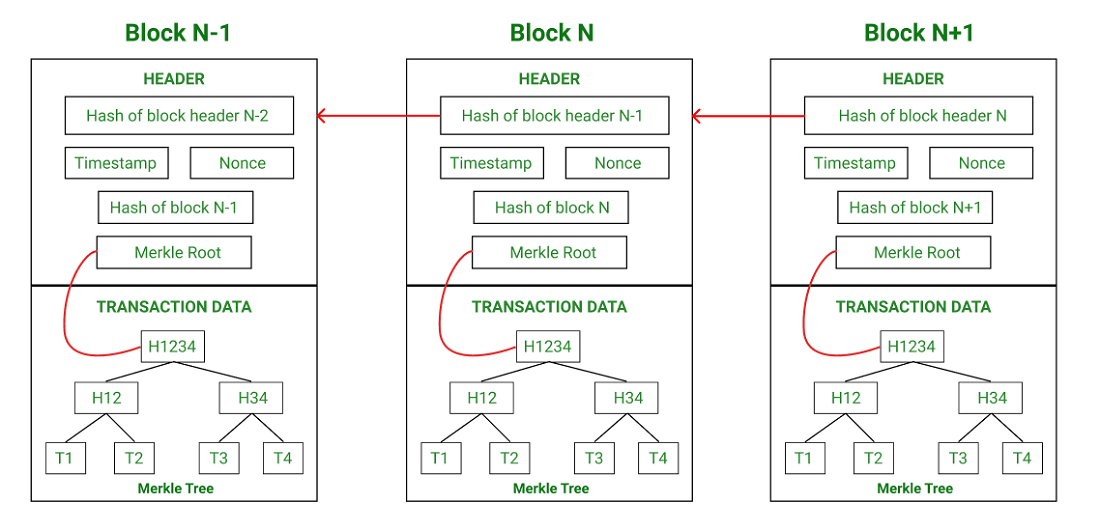
\includegraphics[width=1.1\textwidth]{Blockchain.png}
    \captionsetup{justification=centering}
    \caption{Struttura di una blockchain \cite{Due}}
    \label{fig:blockchain}
\end{figure}
\noindent
Possiamo notare che una blockchain è una linked list di hash pointers in cui:
\begin{itemize}[topsep=5pt, itemsep=0pt]
    \item Ogni blocco è un nodo della lista;
    \item Gli hash pointers collegano il blocco N con il blocco N-1;
    \item Il contenuto di ogni nodo è composto dall'header e dai dati delle transazioni.
\end{itemize}
Analizziamo ora i due componenti fondamentali di ogni blocco.
\begin{itemize}[topsep=5pt, itemsep=0pt]
    \item \textbf{Header}\newline
    L'intestazione di ogni blocco è composta da diverse informazioni. In particolare:
    \begin{itemize}[topsep=-2pt, itemsep=0pt, label={$-$}]
        \item Hash dell'header del blocco precedente e puntatore;
        \item Hash del blocco corrente;
        \item Timestamp e nonce del blocco corrente;
        \item Radice del Merkle Tree delle transazioni del blocco corrente.
    \end{itemize}
    \item \textbf{Dati delle transazioni (Merkle Tree)}\newline
    I dati effettivi delle transazioni sono memorizzati in un Merkle Tree, un particolare albero binario che prende il nome dal suo creatore, Ralph Merkle.\newline
    La necessità di utilizzare un Merkle Tree anziché una semplice linked list di hash pointers è dovuta al fatto che usando una lista sarebbe molto oneroso svolgere alcune operazioni sulle transazioni, come ad esempio verificare se una transazione appartiene ad un determinato blocco. Infatti, oltre a dover scorrere i blocchi uno ad uno, dovremmo passare anche la linked list delle transazioni per ogni blocco!\newline
    L'albero di Merkle, di cui ne esiste uno per blocco, è usato sia per capire se le transazioni di un blocco sono tutte integre (l'errore, in caso ci fosse, si propaga fino alla radice) sia per provare l'appartenenza di una transazione ad un blocco in modo efficiente in termini di tempo.\newline
    \begin{figure}[H]
        \centering
        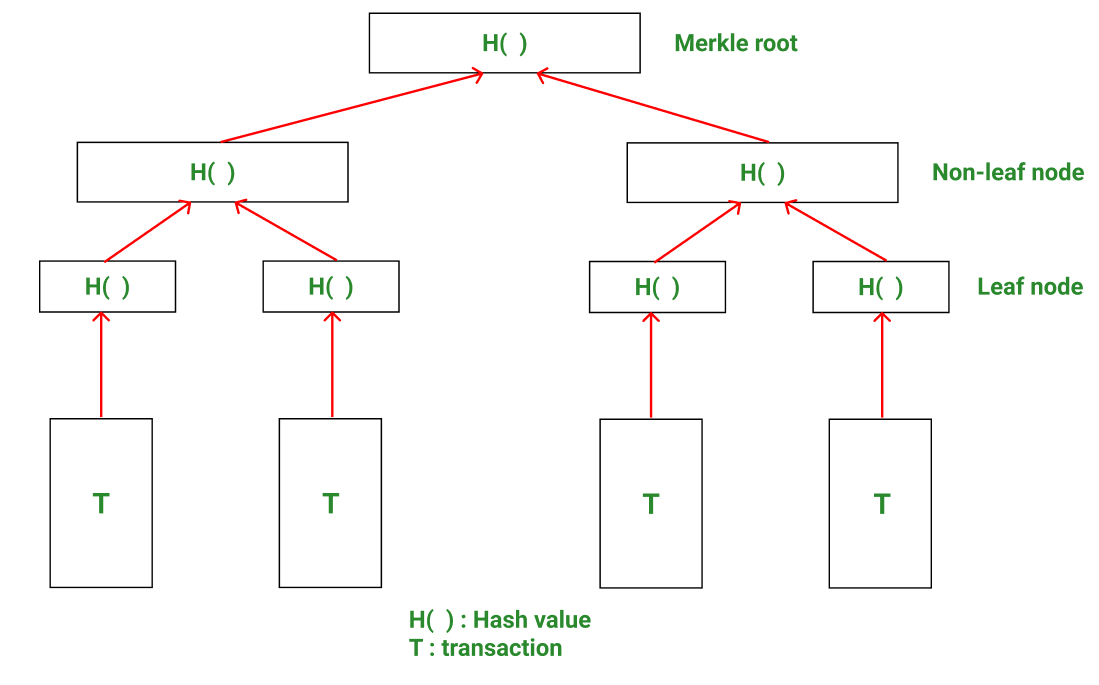
\includegraphics[width=0.9\textwidth]{Merkle.png}
        \captionsetup{justification=centering}
        \caption{Struttura di un Merkle Tree \cite{Due}}
        \label{fig:Merkle}
    \end{figure}
    \newpage
    Osservando la \hyperref[fig:Merkle]{Figura 6} nella pagina precedente, possiamo notare che i Merkle Tree sono costruiti a partire dal basso.\newline
    Inoltre, esistono diversi tipi di nodi:
    \begin{itemize}[topsep=-2pt, itemsep=0pt, label={$-$}]
        \item \textbf{Nodo radice}\newline
        La radice dell'albero di Merkle è memorizzata nell'intestazione del blocco.
        \item \textbf{Nodi non foglia}\newline
        I nodi non foglia, detti anche nodi intermedi, contengono il valore hash dei propri due nodi figli.
        \item \textbf{Nodi foglia}\newline
        I nodi foglia contengono l'hash delle transazioni.
    \end{itemize}
    Le \textbf{transazioni} non sono considerate parte dell'albero.\newline
    Infine, un Merkle Tree è di natura binaria, ossia il numero di nodi foglia deve essere pari affinché l'albero di Merkle sia costruito correttamente. Nel caso in cui ci sia un numero dispari di transazioni, viene semplicemente duplicato l'ultimo hash. \cite{Due} \newpage
\end{itemize}

\section{Smart contract}
Gli smart contracts sono ciò che automatizza effettivamente il lavoro di un notaio. Essi permettono di valutare il successo o il fallimento di una transazione attraverso un codice pre-programmato caricato ed eseguito su una blockchain e basato sui parametri della transazione concordata tra le parti, come il costo degli articoli, dove viene inviato il pagamento e chi autorizza la transazione.\newline
I contratti intelligenti sono necessari per permettere la creazione e il funzionamento di molti componenti del Web 3.0, come gli NFT, le applicazioni decentralizzate e i protocolli di finanza decentralizzata. Ad esempio, uno smart contract è in grado di tenere traccia dei registri di proprietà di un NFT, consentendo di verificare e trasferire facilmente il token da un proprietario ad un altro senza la necessità di un intermediario di terze parti.\newline\newline
Vediamo ora quali sono i vantaggi di utilizzare gli smart contracts:
\begin{itemize}[topsep=5pt, itemsep=0pt]
    \item \textbf{Disponibilità pubblica e sicurezza}\newline
    Gli smart contracts sono registrati sulla blockchain e, quindi, sono pubblicamente disponibili a chiunque possa accedere ad essa. Inoltre, dato che ereditano anche la natura open e decentralizzata della blockchain, possono essere facilmente autenticati.
    \item \textbf{Velocità ed efficienza}\newline
    Dato che gli smart contracts hanno in genere uno scopo specifico possono essere programmati guardando l'efficienza. Le transazioni relative agli smart contracts, quindi, possono essere elaborate rapidamente sulla blockchain.
    \item \textbf{Immutabilità}\newline
    La cronologia di uno smart contract non può essere cancellata o eliminata. \cite{Cinque}
\end{itemize}
\newpage

\section{NFT}
Un NFT (token non fungibile) è un oggetto digitale unico e autentico memorizzato su una blockchain.\newline
Essi sono creati basandosi su uno smart contract caricato in precedenza sulla blockchain che ha il compito di memorizzare tutta la cronologia delle operazioni che si possono svolgere su un NFT, come la creazione o un passaggio di proprietà. \cite{Sei}
\subsection{FT vs NFT}
Qual è la differenza tra un FT (token fungibile) e un NFT (token non fungibile)?\newline
Quando un oggetto è fungibile significa che è intercambiabile con un altro oggetto dello stesso tipo. Un esempio molto semplice è una moneta da 1 Euro: se la si scambiasse con qualcuno, entrambi avrebbero ancora 1 Euro.\newline
Non fungibile, invece, significa che sia l'oggetto sia il suo valore sono assolutamente unici. Un esempio sono due auto della stessa marca e modello: esse, infatti, potrebbero avere valori diversi in base al numero di chilometri percorsi, agli incidenti o al fatto che in precedenza fossero di proprietà di una celebrità. \cite{Sei}
\subsection{Autenticità}
I fatti che tutte le operazioni che si possono svolgere su un NFT sono registrate sulla blockchain e che la chain stessa è accessibile da chiunque sono a tutti gli effetti un certificato di autenticità dell'NFT.\newline
Di norma, infatti, quando si acquista un'opera d'arte o un oggetto da collezione viene fornito anche un certificato di autenticità cartaceo. Esso, però, è spesso perso o distrutto, di fatto rendendo il sistema di garanzia dell'autenticità molto debole.\newline
Le blockchain, invece, offrono una soluzione semplice ma molto più sicura. \cite{Sei}
\subsection{Utilizzi}
Gli NFT possono essere usati per rappresentare oggetti completamente digitali ed essere acquistati a fini collezionistici, ma possono anche essere creati a partire da oggetti fisici realmente esistenti nonché venire associati ad essi: in questo caso prendono il nome di NFT phygital (physical + digital).\newline
Gli NFT phygital hanno davvero molti vantaggi e saranno il punto cardine del sistema che andremo a sviluppare. \cite{Sei} \newpage

\section{Firma digitale}
\label{sec:digitalsignature}
La firma digitale è un metodo che permette di dimostrare importanti proprietà come l’autenticazione del mittente e del destinatario, l’integrità dei dati e la non ripudiabilità di un'operazione. Essa si basa sugli algoritmi di cifratura asimmetrica o a chiave pubblica.\newline
Vediamo un paio di esempi di alcune firme digitali e spieghiamone il funzionamento: supponiamo che un mittente Alice voglia firmare digitalmente un messaggio prima di inviarlo ad un destinatario Bob.
\subsection{RSA Digital Signature}
\begin{enumerate}[topsep=5pt, itemsep=0pt]
    \item Alice genera le seguenti informazioni:
        \begin{itemize}[topsep=-2pt, itemsep=0pt, label={$-$}]
            \item \(p\) e \(q\) numeri primi
            \item \(n = p * q\)
            \item \(e\) con \(MCD(e, \phi(n)) = 1\), con \(\phi(n) =\) numero di coprimi con \(n\)
            \item \(d\) con \(d * e \equiv 1\) MOD \(\phi(n)\)
        \end{itemize}
        (\(e\), \(n\)) formano la chiave pubblica di Alice.\newline
        (\(p\), \(q\), \(d\)) formano la chiave privata di Alice.
    \item Alice pone la propria firma digitale su un messaggio \(m\)\newline
    \(y \equiv m^d\) MOD \(n\)
    \item Alice spedisce (\(m,y\)) a Bob
    \item Bob deve autenticare il messaggio. Quindi calcola \(z \equiv\ y^e\) MOD \(n\)\newline
    Se \(z \equiv m\) MOD \(n\), allora la firma è valida e le proprietà citate in precedenza sono garantite. \cite{Sette}
\end{enumerate}\newpage
\subsection{ElGamal Digital Signature}
\begin{enumerate}[topsep=5pt, itemsep=0pt]
    \item Alice genera le seguenti informazioni:
        \begin{itemize}[topsep=-2pt, itemsep=0pt, label={$-$}]
            \item \(p\) numero primo
            \item \(\alpha\) radice primitiva di \(p\)
            \item \(a\) numero casuale tale che \(a < p - 1\)
            \item \(\beta \equiv \alpha^a\) MOD \(p\)
        \end{itemize}
        (\(p, \alpha, \beta\)) formano la chiave pubblica di Alice.\newline
        \(a\) è la chiave privata di Alice.    
    \item Alice pone la firma digitale seguendo questo metodo
        \begin{itemize}[topsep=-2pt, itemsep=0pt, label={$-$}]
            \item Genera \(k\), un numero segreto tale che \(MCD(k,p-1) = 1\)
            \item Calcola \(r\) ed \(s\)\newline
            \(r \equiv \alpha^k\) MOD \(p\)\newline
            \(s \equiv k^{-1}(m - a * r)\) MOD \(p - 1\)
        \end{itemize}
    \item Alice spedisce (\(m, r, s\)) a Bob
    \item Bob deve autenticare il messaggio. Quindi calcola
        \begin{itemize}[topsep=-2pt, itemsep=0pt, label={$-$}]
            \item \(v1 \equiv \beta^r * r^s\) MOD \(p\)
            \item \(v2 \equiv \alpha^m\) MOD \(p\)
        \end{itemize}
        Se \(v1 \equiv v2\) MOD \(p\), allora la firma è valida e le proprietà citate in precedenza sono garantite. \cite{Sette}
\end{enumerate}

\section{Crypto wallet}
Un crypto wallet è uno strumento virtuale che aiuta ad acquistare, vendere e conservare le criptovalute e gli NFT. In particolare, fornisce un indirizzo blockchain (chiave pubblica) e una chiave privata.\newline
Le criptovalute e gli NFT, inoltre, non sono conservati sul crypto wallet, ma risiedono sempre e solo sulla blockchain: il wallet permette solo di controllarli e gestirli. \cite{Otto}
\subsection{Tipi di crypto wallet}
Esistono due tipi principali di crypto wallet:
\begin{itemize}[topsep=5pt, itemsep=0pt]
    \item \textbf{Custodial o hosted}\newline
    I portafogli sono gestiti da una società terza. È come se la chiave privata del crypto wallet fosse in una struttura sicura che ha il compito di verificare l'identità di chi richiede la chiave prima di fornirla.\newline
    Essi richiedono meno responsabilità, ma c'è un rischio che la propria chiave privata venga rubata in caso di attacchi alla struttura della terza parte.
    \item \textbf{Non custodial o self-custodied}\newline
    I portafogli non sono gestiti da una società terza. È come se la chiave privata del crypto wallet fosse custodita in casa.\newline
    Essi forniscono il pieno controllo sulla propria chiave, ma richiedono una grande attenzione da parte dell'utente, che potrebbe perdere la chiave accidentalmente.\newline
    I portafogli non custodial si dividono ulteriormente in altri due tipi:
    \begin{itemize}[topsep=-2pt, itemsep=0pt, label={$-$}]
        \item \textbf{Portafogli software o hot wallet}\newline
        È un programma che risiede sul proprio computer, dispositivo mobile o sul browser Internet.\newline
        Questo rende i portafogli software un'ottima opzione per acquistare, vendere e trasferire NFT e criptovalute in modo rapido e conveniente.
        \item \textbf{Portafogli hardware o cold wallet}\newline
        È un dispositivo fisico che potrebbe essere necessario collegare al computer per poter essere utilizzato.\newline
        Dato che non è sempre connesso al computer, al dispositivo mobile o al browser, è un'ottima opzione per l'archiviazione sicura a lungo termine, ma è meno conveniente per le transazioni veloci o frequenti.
    \end{itemize}
    Questi wallet, infine, richiedono di impostare una password o un PIN per accedervi. Essa è diversa dalla seed phrase, ossia la frase utilizzata per accedere al wallet in caso di smarrimento della password. \cite{Otto}
\end{itemize}
\subsection{Funzionamento}
Come già detto in precedenza, i crypto wallet forniscono sia un indirizzo blockchain (chiave pubblica) sia una chiave privata. Queste due informazioni sono utilizzate per applicare la firma digitale alle transazioni che saranno caricate sulla blockchain.\newline\newline
La \textbf{chiave privata} ha il compito di dimostrare la proprietà della criptovaluta o dell'NFT archiviato in uno specifico indirizzo blockchain pubblico.\newline
Essa è una stringa di caratteri (in genere 64) generata in modo casuale. È tenuta segreta e serve per controllare il wallet e tutto ciò che è memorizzato presso il relativo indirizzo pubblico.\newline\newline
L'\textbf{indirizzo pubblico} è una lunga stringa di caratteri che identifica le operazioni di ogni utente sulla blockchain, nonché l'informazione conosciuta da tutti gli altri utenti se volessero interagire con noi ad esempio per scambi, acquisti o vendite di criptovalute ed NFT.\newline
Sulla blockchain di Ethereum e su quelle EVM-compatibili (vedi \hyperref[sec:EVM]{Sezione 3.1}) si tratta di una serie di 42 caratteri che iniziano con "0x" come prefisso.\newline\newline
Si utilizzano quindi degli algoritmi per apporre la firma digitale sulla transazione.\newline
Il funzionamento è molto semplice: l'utente firma digitalmente la transazione con la propria chiave privata ed essa sarà verificata utilizzando l'indirizzo pubblico dell'utente, ossia la sua chiave pubblica. \cite{Otto} \newpage

\section{Blockchain explorer}
I blockchain explorer sono dei particolari siti che consentono agli utenti di cercare, confermare e convalidare facilmente le transazioni che vengono memorizzate sulla blockchain a cui fanno riferimento. Questi strumenti possono essere utilizzati da chiunque, dagli sviluppatori ai proprietari degli NFT.\newline
Andiamo nel dettaglio dei servizi offerti da questi explorer:
\begin{itemize}[topsep=5pt, itemsep=0pt]
    \item \textbf{Funzionalità di ricerca}: i blockchain explorer consentono agli utenti di cercare indirizzi sulla blockchain. Essi possono mostrare, ad esempio, la cronologia delle transazioni, i saldi dei token e le interazioni con gli smart contracts. Analogamente ai motori di ricerca, è presente una barra in cui gli utenti possono digitare la transazione o le chiavi hash che stanno cercando.
    \item \textbf{Monitoraggio delle transazioni}: i blockchain explorer consentono agli utenti di visualizzare e tracciare le transazioni in tempo reale. Gli utenti possono vedere dettagli come l'hash della transazione, gli indirizzi del mittente e del destinatario, i gas fees e lo stato della transazione.
    \item \textbf{Analisi degli smart contracts}: i blockchain explorer consentono agli utenti di visualizzare il codice sorgente, il bytecode e la cronologia delle transazioni degli smart contracts, nonché permettere una serie di operazioni come il trasferimento di proprietà degli NFT.
    \item \textbf{Monitoraggio dei token}: i blockchain explorer consentono agli utenti di controllare la situazione dei token, tra cui anche chi li detiene e il volume degli scambi nelle ultime 24 ore.
    \item \textbf{Statistiche di rete}: i blockchain explorer forniscono agli utenti le statistiche della rete in tempo reale e alcuni dati storici sulle sue prestazioni passate. \cite{Nove}
\end{itemize}
Alcuni esempi di blockchain explorer sono \href{https://etherscan.io/}{Etherscan} \cite{Dieci} per la blockchain Ethereum e \href{https://polygonscan.com/}{PolygonScan} \cite{Undici} per la blockchain Polygon.

\chapter{Scelta della blockchain}
\noindent
Prima di addentrarci nell’analisi del sistema di protezione, è necessario compiere alcune considerazioni su alcune scelte preliminari effettuate durante l’ideazione del metodo vero e proprio.\newline
La prima è la seguente: visto l’elevatissimo numero di blockchain esistenti, è assolutamente necessario scegliere quella che più si adatta alle caratteristiche del nostro progetto, seguendo una serie di criteri di selezione.
\section{Compatibilità con EVM}
\label{sec:EVM}
Il primo criterio utilizzato è stato quello di scegliere una blockchain EVM-compatibile.\newline
EVM, acronimo di Ethereum Virtual Machine, è un ambiente software che ha il compito di eseguire tutte le operazioni e le transazioni sulla blockchain di Ethereum: archivia i dati sulla blockchain, elabora le transazioni e calcola i gas fees.\newline
L'EVM è una virtual machine Turing-completa, ossia è in grado di eseguire qualsiasi algoritmo o programma. Il vantaggio di ciò è che Ethereum è ampiamente programmabile, ossia che degli sviluppatori possono scrivere comodamente degli smart contracts e delle applicazioni decentralizzate ed eseguirli sulla rete Ethereum.\newline
L'EVM, inoltre, esegue il codice in modo deterministico: ogni smart contract produrrà sempre lo stesso output dato lo stesso input, indipendentemente da dove viene eseguito o da chi lo sta eseguendo. Questa proprietà garantisce che gli smart contracts vengano eseguiti senza interferenze da fonti esterne.\newline
L'EVM è progettato per essere isolato dal resto del sistema operativo del computer. Questo implica che l'EVM può interagire solo con la rete Ethereum, impedendo ai malintenzionati di accedere al sistema sottostante o di compromettere la sicurezza della rete.\newpage

\noindent
Fatta questa doverosa premessa, cosa significa e che vantaggi dà il fatto di utilizzare una blockchain EVM-compatibile?\newline
La compatibilità EVM si riferisce alla capacità di una blockchain di eseguire l'EVM e gli smart contracts di Ethereum. Una blockchain EVM-compatibile garantisce quindi dei notevoli vantaggi per gli sviluppatori e non solo:
\begin{itemize}[topsep=5pt, itemsep=0pt]
    \item Essendo Ethereum una delle blockchain più popolari, è molto più semplice trovare online la soluzione ad eventuali problematiche riscontrate durante lo sviluppo delle applicazioni decentralizzate e degli smart contracts, nonché eventuali plugin ed estensioni che rendono lo sviluppo più semplice e veloce.
    \item Le applicazioni decentralizzate e gli smart contracts sviluppati per una blockchain compatibile con EVM possono essere facilmente migrati su altre blockchain compatibili con EVM con modifiche minime al codice.
    \item L'EVM fornisce un ambiente standardizzato per scrivere smart contracts e sviluppare applicazioni decentralizzate: ciò significa che posso scrivere tutto il codice in Solidity, uno dei linguaggi di programmazione più utilizzati per Ethereum, e di seguito adattarlo a più situazioni con costi veramente molto bassi.
    \item Gli smart contracts e le applicazioni decentralizzate sviluppate su blockchain EVM-compatibili sono costruite sulla rete Ethereum per natura, il che significa che sono automaticamente disponibili ai milioni di wallet collegati ad essa. \cite{Dodici}
\end{itemize}

\section{Ecosostenibilità}
Il secondo criterio utilizzato è stato quello di scegliere una blockchain eco-friendly. In particolare, ci siamo concentrati sulla ricerca di una blockchain che permetta di risparmiare il più possibile in termini di consumi elettrici e di emissioni di anidride carbonica. Dopo un'attenta ricerca in rete, abbiamo individuato uno studio dell'ottobre 2022 del Crypto Carbon Ratings Institute (CCRI) \cite{Tredici}, una compagnia di ricerca tedesca che si occupa di studiare e fornire dati sugli aspetti sostenibili delle blockchain e delle criptovalute.

\begin{table}[H]
\centering
\begin{tabular}{|c|c|}
\hline
\textbf{Blockchain/Entità} & \textbf{Consumo elettrico annuo [kWh]} \\
\hline
Famiglia statunitense & 10'600 \\
\hline
Polkadot & 70'246 \\
\hline
Polygon & 118'934 \\
\hline
Tezos & 123'500 \\
\hline
Tron & 160'210 \\
\hline
Avalanche & 592'240 \\
\hline
Cardano & 638'488 \\
\hline
Algorand & 721'187 \\
\hline
Ethereum post-Merge & 2'105'304 \\
\hline
Solana & 3'900'968 \\
\hline
Ethereum pre-Merge & 21'986'314'331 \\
\hline
Bitcoin & 97'111'432'951 \\
\hline
\end{tabular}
\captionsetup{justification=centering}
\caption{Consumo elettrico annuo [kWh] di varie blockchain confrontato con quello di una famiglia statunitense \cite{Tredici}}
\label{tab:elettricità}
\end{table}

\begin{figure}[H]
    \centering
    \includegraphics[width=1.1\textwidth]{Elettricità.png}
    \captionsetup{justification=centering}
    \caption{Consumo elettrico annuo [kWh] di varie blockchain confrontato con quello di una famiglia statunitense \cite{Tredici}}
    \label{fig:elettricità}
\end{figure}

\begin{table}[H]
\centering
\begin{tabular}{|c|c|}
\hline
\textbf{Blockchain/Entità} & \textbf{Emissioni di CO2 annue [tonnellate]} \\
\hline
Volo intercontinentale & 6.1 \\
\hline
Polkadot & 33.37 \\
\hline
Polygon & 55.0 \\
\hline
Tezos & 58.66 \\
\hline
Tron & 76.1 \\
\hline
Avalanche & 281.31 \\
\hline
Cardano & 303.28 \\
\hline
Algorand & 342.56 \\
\hline
Ethereum post-Merge & 704.055 \\
\hline
Solana & 1852.96 \\
\hline
\end{tabular}
\captionsetup{justification=centering}
\caption{Emissioni di CO2 annue [tonnellate] di varie blockchain confrontate con quelle di un volo in business class da Monaco di Baviera e San Francisco \cite{Tredici}}
\label{tab:CO2}
\end{table}

\begin{figure}[H]
    \centering
    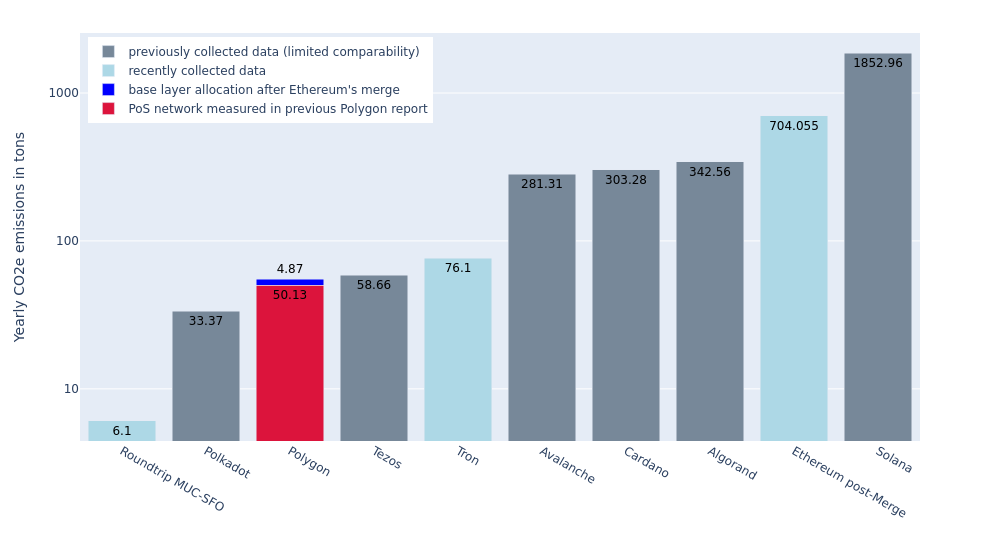
\includegraphics[width=1.1\textwidth]{CO2.png}
    \captionsetup{justification=centering}
    \caption{Emissioni di CO2 annue [tonnellate] di varie blockchain confrontate con quelle di un volo in business class da Monaco di Baviera e San Francisco \cite{Tredici}}
    \label{fig:CO2}
\end{figure}\newpage

\noindent
Osserviamo i dati riguardanti i consumi elettrici: il primo fatto che salta all'occhio è sicuramente l'enorme differenza di elettricità consumata dalla blockchain di Bitcoin e quella di Ethereum pre-Merge, ossia prima che diventasse una blockchain Proof-of-Stake, rispetto a tutte le altre. Questo ci fa comprendere quanto scegliere una blockchain green sia realmente importante.\newline
Inoltre, si può notare anche la netta differenza tra il consumo elettrico di una famiglia statunitense rispetto alle blockchain che consumano di meno. Questo ci permette di concludere che, al momento, la tecnologia blockchain è ancora molto esosa in termini di risorse elettriche, anche se si sta lavorando molto per ridurre questo aspetto.\newline\newline
Per quanto riguarda le emissioni di CO2 il discorso è molto simile a quello fatto per il consumo elettrico. Anche qui, infatti, ci sono delle blockchain che emettono significativamente molta più CO2 rispetto alle altre, vedasi Solana ed Ethereum post-Merge, così come è vero che anche le blockchain che emettono meno anidride carbonica inquinano molto di più l'ambiente rispetto ad un volo intercontinentale in business class.\newpage

\section{Identificazione della blockchain}
\label{sec:polygon}
Dopo un'attenta analisi, la scelta della blockchain è ricaduta su Polygon.\newline
Polygon è una blockchain creata per ridurre i costi di transazione di Ethereum e migliorarne la velocità complessiva. A causa della sua popolarità, infatti, Ethereum ha dei tempi di transazione e dei gas fees parecchio elevati. Inoltre, Polygon ha un token nativo, il MATIC, e utilizza il metodo di convalida Proof-of-Stake.\newline
Polygon è una sidechain di Ethereum. Come spiegato in precedenza, le sidechain sono delle blockchain layer 2 collegate ad una blockchain layer 1 tramite un bridge bidirezionale, ma separate e indipendenti da essa. Tra le varie competenze, esse sono in grado di ricevere del lavoro da svolgere dalla blockchain principale e, dopo averlo compiuto, restituiscono unicamente i risultati, permettendo di guadagnare in termini di efficienza.\newline\newline
Oltre alle caratteristiche appena descritte, Polygon soddisfa molto bene i due criteri di selezione che abbiamo definito. Infatti, oltre ad essere una blockchain EVM-compatibile ed avere uno stretto legame con Ethereum, è una delle più attente all'ambiente (vedi \hyperref[tab:elettricità]{Tabella 1}, \hyperref[fig:elettricità]{Figura 7}, \hyperref[tab:CO2]{Tabella 2} e \hyperref[fig:CO2]{Figura 8}).\newline
Se ciò non bastasse, sulla pagina web \cite{Quattordici} è possibile osservare che la sostenibilità e il bene del pianeta sono due  obiettivi cardine del progetto Polygon.\newpage

\chapter{Scelta dell'approccio}
\label{chap:capitolo4}
\noindent
Una volta selezionata la blockchain sulla quale far vivere il nostro sistema, una seconda scelta necessaria riguarda la cardinalità degli NFT. Dato che una parte essenziale del metodo prevede il minting di NFT, ossia la loro creazione e il loro conio sulla blockchain, è assolutamente fondamentale capire quanti e quali NFT creare, in particolare per i casi in cui ho tante copie di un bene da proteggere.\newline
Facciamo un esempio per chiarire il problema: supponiamo di voler proteggere un orologio di lusso
\begin{itemize}[topsep=5pt, itemsep=0pt]
    \item Se l'orologio fosse prodotto in un'unica copia, allora sarebbe sufficiente creare un unico NFT e associarlo all'orologio.
    \item Se l'orologio fosse prodotto in più copie indistinguibili tra loro, invece, la situazione sarebbe più interessante: è meglio creare un unico NFT e associarlo a tutte le copie oppure conviene mintare un NFT per ogni singola copia dell'orologio?
\end{itemize}
È semplice intuire che esistono due modi di agire: l'approccio 1:N e l'approccio 1:1.\newline
Analizziamo nel dettaglio le caratteristiche, i pro e i contro di ognuno di essi.\newpage

\section{Approccio 1:N}
L'approccio 1:N di creazione degli NFT è il più semplice e meno dispendioso in termini di risorse. Esso prevede semplicemente di creare un unico NFT e associarlo a tutte le copie dell'oggetto.\newline
Sebbene questo metodo permetta di risparmiare molte risorse in caso un oggetto sia prodotto in un gran numero di copie, ha anche il grande svantaggio di essere molto vulnerabile alle truffe. Per via del fatto che non è chiaramente possibile trasferire l'NFT all'effettivo proprietario dell'oggetto fisico dopo la prima vendita, è molto complesso trovare un metodo per associare in modo sicuro l'NFT al bene senza che un potenziale truffatore copi il metodo di associazione e lo apponga su un oggetto fasullo. Un banale QR code, ad esempio, non sarebbe assolutamente sufficiente, e questo ci costringerebbe a cercare un metodo di associazione molto più complesso.

\section{Approccio 1:1}
\label{sec:1to1}
L'approccio 1:1 di creazione degli NFT è invece più oneroso e leggermente più complesso. Prevede, infatti, di creare un NFT per ogni oggetto effettivo: se l'orologio dell'esempio precedente fosse prodotto in 1000 copie, allora sarà necessario creare 1000 NFT e numerarli come "Orologio \#1", "Orologio \#2", etc.\newline
A differenza dell'approccio 1:N, ora abbiamo un'associazione univoca tra NFT e oggetto fisico: questo ci permette di trasferire l'NFT all'effettivo proprietario del bene ogni qualvolta esso viene venduto. Grazie a questa proprietà, come spiegato più chiaramente nella \hyperref[sec:idea1]{Sezione 6.1}, è sufficiente un semplicissimo QR code come metodo di associazione.\newpage
\noindent
Il problema di questo approccio, però, è che richiede una grande quantità di risorse sotto tre principali aspetti:
\begin{itemize}[topsep=5pt, itemsep=0pt]
    \item \textbf{Soldi}\newline
    Assumendo un costo dei gas fees di Polygon di circa 0.01\$, creare 100.000 NFT ha un costo base di 1000\$, una cifra che potrebbe essere poco sostenibile per il piccolo artigiano locale, scoraggiandolo dal voler utilizzare il sistema da noi ideato.\newline
    Tuttavia, si può assumere che un numero così grande di NFT sarà richiesto esclusivamente da grandi aziende che, di conseguenza, non avrebbero problemi a spendere una cifra medio-alta per garantire protezione ai loro prodotti.
    \item \textbf{Spazio}\newline
    Creando una grande quantità di NFT occuperemo molto spazio sulla blockchain, ma anche questo non è un problema visto che, se non per delle limitazioni tecniche, le blockchain hanno una capacità potenzialmente illimitata.\newline
    Un problema leggermente più grave, tuttavia, è il fatto che potrebbero essere caricati inutilmente sulla blockchain NFT di beni che rimarranno invenduti.
    \item \textbf{Tempo}\newline
    Il principale problema dell'approccio 1:1 di creazione degli NFT è il seguente: assumendo un tempo di circa 15 secondi per il minting di un NFT su Polygon e senza considerare eventuali conflitti o errori, il tempo per caricare, ad esempio, 200.000 NFT è di circa 34 giorni!
\end{itemize}
Per mascherare i problemi rimasti in termini di tempo e spazio, una possibile soluzione può essere di creare gli NFT dinamicamente a mano a mano che gli oggetti fisici vengono venduti (vedi \hyperref[sec:vendere]{Sezione 6.3}).\newpage

\section{Definizione dell'approccio corretto}
Analizzati i pro e i contro descritti in questo capitolo, abbiamo optato per l'adozione dell'approccio 1:1.\newline
La motivazione di questa scelta è legata al principale svantaggio che l'approccio 1:N porta con sè. Esso è molto grave e rischierebbe di danneggiare l'intero sistema rendendolo sostanzialmente inutilizzabile. Gli svantaggi dell'approccio 1:1, invece, sono mascherabili, mentre i suoi vantaggi sono particolarmente importanti.\newline
Oltre a questa motivazione c'è anche una questione semantica. Gli NFT sono stati progettati per rappresentare oggetti unici nel loro genere, perciò utilizzare un NFT per rappresentare più oggetti fisici è una contraddizione. Al contrario, è preferibile distinguere i beni prodotti in più copie attraverso l'uso di numeri incrementali, in modo da renderli effettivamente unici (ad esempio: non esisteranno mai due oggetti "Orologio \#1").

\chapter{Il metodo}
\label{chap:metodo}
\noindent
Siamo finalmente giunti alla descrizione del metodo vero e proprio, ossia il sistema per proteggere un qualsiasi bene come precedentemente descritto.\newline
Si noti che questo metodo, nei dettagli implementativi che saranno forniti, è garantito funzionare solo con blockchain EVM-compatibili, in particolare con Polygon.\newline
La sua struttura generale, tuttavia, si può prendere come modello per \textit{\textbf{qualsiasi}} altro caso d'uso, quindi non solo in termini di blockchain diverse.
\section{Documento di specifica per il cliente}
\label{sec:documento}
\noindent
La prima fase prevede la definizione di un documento di specifica per il cliente.\newline
In questo documento sono elencate tutte le informazioni che il cliente (o un suo delegato) deve produrre ed esibire affinché si possa creare un NFT rappresentante un bene materiale di cui è proprietario.\newline
Qui di seguito sono elencati tutti i passi necessari alla stesura del documento.
\subsection{Identificazione del cliente}
Il cliente (o un suo delegato) deve presentare delle prove che attestino la sua identità.\newline
Questo passo è necessario per evitare che qualsiasi persona possa commissionare la creazione di NFT fingendosi qualcun altro.\newline
\textbf{Esempi:} bigliettino da visita, pagina LinkedIn, contratto di assunzione, ...\newpage
\subsection{Certificato di autenticità del prodotto}
Il cliente (o un suo delegato) deve presentare un documento fisico o digitale che attesti che il prodotto su cui si vuole creare un NFT è di sua proprietà (o della persona da cui è stato delegato). Si noti bene che verrà archiviata una copia firmata di questo documento.\newline
Questo passo è necessario per evitare che qualsiasi persona possa commissionare la creazione di NFT su prodotti dei quali non possiede il diritto di proprietà.\newline
\textbf{Esempi contenuto:} certificato di un ente ufficiale, marchio registrato, ...\newline
\textbf{Esempi formato:} cartaceo, PDF, ...
\begin{figure}[H]
    \centering
    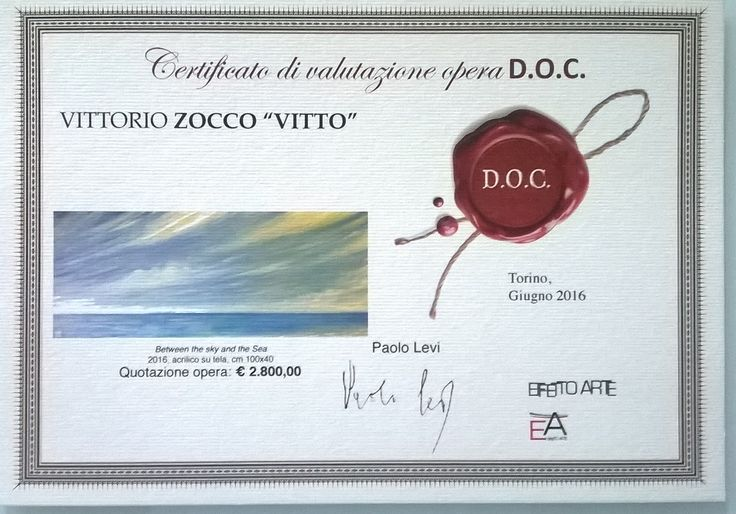
\includegraphics[width=1\textwidth]{Certificate.jpeg}
    \captionsetup{justification=centering}
    \caption{Esempio di certificato di autenticità \cite{Quindici}}
    \label{fig:certificato}
\end{figure}

\subsection{Scheda del prodotto}
Il cliente (o un suo delegato) deve presentare un documento fisico o digitale in cui siano elencate delle caratteristiche fondamentali dell'oggetto che lo rendono unico e riconoscibile. Queste informazioni diverranno i metadati dell'NFT.\newline
\textbf{Esempi formato:} cartaceo, PDF, DOC, DOCX, ...
\subsection{Rappresentazione grafica del prodotto}
Il cliente (o un suo delegato) deve presentare un'immagine statica o animata che rappresenterà l'NFT insieme ai metadati descritti nel punto precedente.\newline
\textbf{Esempi formato:} JPG, PNG, GIF, ...\newline
\textbf{Esempio immagine:} si veda la \hyperref[fig:DG]{Figura 10}
\begin{figure}[H]
    \centering
    
\includegraphics[width=0.7\textwidth]{DG.jpg}
    \captionsetup{justification=centering}
    \caption{Esempio di immagine \cite{Sedici}}
    \label{fig:DG}
\end{figure}

\section{Operazioni preliminari}
Dopo aver raccolto tutte le informazioni necessarie dal cliente, la seconda fase prevede di svolgere una serie di operazioni in vista delle fasi successive.\newline
Entrando nel dettaglio, le operazioni sono le seguenti:
\begin{itemize}[topsep=5pt, itemsep=0pt]
    \item Accedere ad Alchemy \cite{Diciassette}, una piattaforma per blockchain developers che fornisce un’interfaccia per comunicare facilmente con alcune blockchain;
    \item Autenticatsi su un crypto wallet a scelta. In particolare, noi abbiamo utilizzato MetaMask \cite{Diciotto}.
\end{itemize}
Durante lo sviluppo del sistema, inoltre, è stata utilizzata Polygon Mumbai, una Testnet di Polygon, e il sito web \cite{Diciannove} per la generazione di MATIC da utilizzare su Mumbai.\newline
Nei prossimi punti, invece, descriveremo il metodo finale usando la Polygon Mainnet.\newpage

\section{Creazione di uno smart contract}
\label{sec:contratto}
Siamo giunti finalmente alla fase di scrittura dello smart contract che ci servirà successivamente per mintare gli NFT.\newline
In particolare, i passi da seguire sono i seguenti:
\begin{enumerate}[topsep=5pt, itemsep=0pt]

\item \textbf{Creare una nuova app in Alchemy}\newline
Per facilitare lo sviluppo dello smart contract e il minting degli NFT, iniziamo creando una nuova app in Alchemy, selezionando in particolare la blockchain e la rete sulle quali caricheremo lo smart contract e, di conseguenza, gli NFT.\newline
Nel nostro caso, quindi, sceglieremo come blockchain \textit{\textbf{Polygon PoS}} e come rete \textit{\textbf{Polygon Mainnet}}.

\item \textbf{Creare un nuovo progetto in locale}\newline
È necessario creare una nuova cartella nel file system locale. In essa verrà inserito tutto il progetto che stiamo costruendo.\newline
Una volta creata, spostiamoci in essa ed eseguiamo da riga di comando
\begin{lstlisting}[language=HTML, numbers=none, aboveskip=2pt, belowskip=-3pt]
npm init
\end{lstlisting}
npm è un gestore di pacchetti per JavaScript, uno dei linguaggi di programmazione che utilizzeremo in seguito.

\item \textbf{Installare Hardhat}\newline
Eseguiamo da riga di comando
\begin{lstlisting}[language=HTML, numbers=none, aboveskip=2pt, belowskip=-3pt]
npm install --save-dev hardhat
\end{lstlisting}
per installare Hardhat, un ambiente di sviluppo che aiuta a compilare, debuggare e testare lo smart contract localmente prima di pubblicarlo sulla blockchain.\newpage

\item \textbf{Creare un progetto Hardhat}\newline
Eseguiamo da riga di comando
\begin{lstlisting}[language=HTML, numbers=none, aboveskip=2pt, belowskip=-3pt]
npx hardhat init
\end{lstlisting}
e successivamente selezioniamo l'opzione
\begin{lstlisting}[language=HTML, numbers=none, aboveskip=2pt, belowskip=-3pt]
Create an empty hardhat.config.js
\end{lstlisting}
Questo permetterà di creare un nuovo progetto Hardhat.

\item \textbf{Aggiungere cartelle per organizzare meglio il progetto}\newline
All'interno della cartella del nostro progetto creiamo la cartella \textit{\textbf{contracts}}, che conterrà il codice dello smart contract, e la cartella \textit{\textbf{scripts}}, che includerà i codici JavaScript che permetteranno di operare con lo smart contract.

\item \textbf{Scrivere il codice dello smart contract in Solidity}\newline
Attraverso il comando
\begin{lstlisting}[language=HTML, numbers=none, aboveskip=2pt, belowskip=-3pt]
npm install @openzeppelin/contracts@^4.9.3
\end{lstlisting}
includiamo nel nostro progetto una libreria che ci servirà in seguito.\newline
Successivamente è arrivato il momento di scrivere il codice dello smart contract in un file \textit{\textbf{X.sol}} (con X a scelta) e di salvarlo all'interno della cartella \textit{\textbf{contracts}}.\newline
Qui di seguito è riportato un codice d'esempio di uno smart contract.
\begin{lstlisting}[language=Solidity, aboveskip=2pt]
// Contract based on [https://docs.openzeppelin.com/contracts/3.x/erc721]
// SPDX-License-Identifier: MIT

// Versione di Solidity utilizzata
pragma solidity ^0.8.21;

import "@openzeppelin/contracts/token/ERC721/ERC721.sol";
import "@openzeppelin/contracts/token/ERC721/extensions/ERC721URIStorage.sol";
import "@openzeppelin/contracts/utils/Counters.sol";
import "@openzeppelin/contracts/access/Ownable.sol";

// Definizione dello smart contract
contract Contract is ERC721URIStorage, Ownable {

    // Dichiarazione del contatore per gli ID
    using Counters for Counters.Counter;
    Counters.Counter private _tokenIds;

    // Costruttore (nome del contratto, simbolo del contratto)
    // Il nome e' quello che comparira' sul crypto wallet
    constructor() ERC721("Esempio", "NFT") {}

    // Funzione che permette di coniare un nuovo NFT da questo smart contract
    // recipient: indirizzo che ricevera' l'NFT coniato
    // tokenURI: collegamento ad un file JSON che contiene i metadati dell'NFT coniato
    function mintNFT(address recipient, string memory tokenURI) public onlyOwner returns (uint256) {
        // Incrementa il contatore
        _tokenIds.increment();
        // Conia il nuovo NFT
        uint256 newItemId = _tokenIds.current();
        _mint(recipient, newItemId);
        _setTokenURI(newItemId, tokenURI);
        // Restituisce l'ID del nuovo NFT
        return newItemId;
    }
}
\end{lstlisting}

\item \textbf{Collegare Alchemy e il crypto wallet al progetto}\newline
Dopo aver eseguito da riga di comando
\begin{lstlisting}[language=HTML, numbers=none, aboveskip=2pt, belowskip=-3pt]
npm install dotenv -save
\end{lstlisting}
creiamo un file di configurazione \textit{\textbf{.env}} all'interno della cartella del progetto.\newline
Esso deve contenere le seguenti informazioni
\begin{lstlisting}[language=HTML, numbers=none, aboveskip=2pt]
# APIKey HTTPS dell'app su Alchemy
API_URL = "https://polygon-mumbai.g.alchemy.com/v2/abcdefghijk"

# Chiave privata del crypto wallet
PRIVATE_KEY = "0123456789"
\end{lstlisting}\newpage

\item \textbf{Installare hardhat-ethers}\newline
Eseguendo da riga di comando
\begin{lstlisting}[language=HTML, numbers=none, aboveskip=2pt, belowskip=-3pt]
npm install --save-dev @nomiclabs/hardhat-ethers ethers@^5.0.0
\end{lstlisting}
si include hardhat-ethers nel proprio progetto, un plugin che rende più semplice interagire ed effettuare richieste alle blockchain EVM. Esso wrappa i metodi JSON-RPC standard, permettendo di interagire con la blockchain con dei metodi più user-friendly.

\item \textbf{Aggiornare hardhat.config.js}\newline
Il file \textit{\textbf{hardhat.config.js}} contiene un riassunto delle caratteristiche del contratto e dei plugin utilizzati da esso.\newline
In particolare, va aggiornato come segue:
\begin{lstlisting}[language=JavaScript, aboveskip=2pt]
require('dotenv').config();
require("@nomiclabs/hardhat-ethers");

const {API_URL, PRIVATE_KEY} = process.env;

module.exports = {
   solidity: "0.8.21",
   defaultNetwork: "polygon_mainnet",
   networks: {
      hardhat: {},
      polygon_mainnet: {
         url: API_URL,
         accounts: [`0x${PRIVATE_KEY}`]
      }
   }
}
\end{lstlisting}\newpage

\item \textbf{Scrivere lo script deploy.js}\newline
Questo script JavaScript serve per distribuire il contratto, ossia per caricarlo sulla blockchain scelta, nel nostro caso Polygon.\newline
Ricordarsi di inserire il file \textit{\textbf{deploy.js}} all'interno della cartella \textit{\textbf{scripts}}.\newline
Qui di seguito il codice.
\begin{lstlisting}[language=JavaScript, aboveskip=2pt]
async function main() {

    // Crea un "fabbricatore di istanze" dello smart contract
    const MyNFT = await ethers.getContractFactory("Contract")
  
    // Crea una nuova istanza dello smart contract
    const myNFT = await MyNFT.deploy()
    await myNFT.deployed()
    console.log("Contratto distribuito all'indirizzo:", myNFT.address)
}
  
// Esecuzione di main e cattura errori
main()
  .then(() => process.exit(0))
  .catch((error) => {
    console.error(error)
    process.exit(1)
})
\end{lstlisting}

\item \textbf{Distribuire il contratto eseguendo lo script}\newline
Eseguiamo da riga di comando
\begin{lstlisting}[language=HTML, numbers=none, aboveskip=2pt, belowskip=-3pt]
npx hardhat --network "nomeRete" run scripts/deploy.js
\end{lstlisting}
Nel nostro caso, quindi, il comando da eseguire è
\begin{lstlisting}[language=HTML, numbers=none, aboveskip=2pt, belowskip=-3pt]
npx hardhat --network polygon_mainnet run scripts/deploy.js
\end{lstlisting}

\end{enumerate}\newpage

\section{Verifica dello smart contract}
Dopo aver caricato il contratto sulla blockchain, la fase successiva è la sua verifica.\newline
Questa fase consiste nel confrontare il codice sorgente originale del contratto con il bytecode compilato che viene effettivamente eseguito sulla blockchain.\newline
Questo processo è molto importante perché il codice del contratto pubblicato potrebbe essere diverso da quello effettivamente eseguito sulla blockchain, a causa, ad esempio, di errori nella compilazione o di manipolazioni malevole.\newline
Inoltre, verificare lo smart contract ci darà successivamente la possibilità di eseguire delle importanti operazioni su PolygonScan in modo molto più user-friendly.\newline
I passi da seguire per verificare il contratto, quindi, sono i seguenti:
\begin{enumerate}[topsep=5pt, itemsep=0pt]

\item \textbf{Installare hardhat-verify}\newline
Eseguiamo da riga di comando
\begin{lstlisting}[language=HTML, numbers=none, aboveskip=2pt, belowskip=-3pt]
npm install --save-dev @nomicfoundation/hardhat-verify
\end{lstlisting}
per installare hardhat-verify, un plugin che aiuta gli sviluppatori a verificare gli smart contract sulle blockchain EVM-compatibili.

\item \textbf{Aggiornare .env}\newline
Aggiungiamo a \textit{\textbf{.env}} una variabile contenente una API Key di PolygonScan.\newline
Per ottenere una API Key si visiti la seguente pagina web: \cite{Venti}.\newline
Il codice di \textit{\textbf{.env}}, quindi, risulta essere il seguente:
\begin{lstlisting}[language=HTML, numbers=none, aboveskip=2pt]
# APIKey HTTPS dell'app su Alchemy
API_URL = "https://polygon-mumbai.g.alchemy.com/v2/abcdefghijk"

# Chiave privata del crypto wallet
PRIVATE_KEY = "0123456789"

# APIKey di PolygonScan
API_KEY = "kjihgfedcba"
\end{lstlisting}\newpage

\item \textbf{Aggiornare hardhat.config.js}\newline
Aggiorniamo \textit{\textbf{hardhat.config.js}} con le ultime novità.
\begin{lstlisting}[language=JavaScript, aboveskip=2pt]
require('dotenv').config();
require("@nomiclabs/hardhat-ethers");
require("@nomicfoundation/hardhat-verify");

const {API_URL, PRIVATE_KEY, API_KEY} = process.env;

module.exports = {
   solidity: "0.8.21",
   defaultNetwork: "polygon_mainnet",
   networks: {
      hardhat: {},
      polygon_mainnet: {
         url: API_URL,
         accounts: [`0x${PRIVATE_KEY}`]
      }
   },
   etherscan: {
      apiKey: {
         polygon_mainnet: API_KEY
      }
   }
}
\end{lstlisting}

\item \textbf{Verificare il contratto}\newline
Eseguiamo da riga di comando
\begin{lstlisting}[language=HTML, numbers=none, aboveskip=2pt, belowskip=-3pt]
npx hardhat verify --network "nome rete" "indirizzo contratto"
\end{lstlisting}
Nel nostro caso, quindi, il comando da eseguire è
\begin{lstlisting}[language=HTML, numbers=none, aboveskip=2pt]
npx hardhat verify --network polygon_mainnet 0x123456789
\end{lstlisting}
\end{enumerate}\newpage

\section{Creazione degli NFT}
Abbiamo creato, caricato sulla blockchain e verificato uno smart contract. La fase successiva prevede di utilizzare il contratto intelligente per mintare gli NFT secondo l'approccio definito nel \hyperref[chap:capitolo4]{Capitolo 4}. Procediamo con l'analisi dei passi da seguire:
\begin{enumerate}[topsep=5pt, itemsep=0pt]

\item \textbf{Decentralizzare l'immagine e i metadati dell'NFT}\newline
Per questo punto utilizzeremo \href{https://www.pinata.cloud/}{Pinata} \cite{Ventuno}, un sito che permette di caricare file sull'InterPlanetary File System (IPFS), una rete peer-to-peer che permette di archiviare e condividere dati in un file system distribuito. Questo sito servirà per decentralizzare alcune delle informazioni raccolte nel Documento di specifica per il cliente (vedi \hyperref[sec:documento]{Sezione 5.1}). In particolare:
\begin{itemize}[topsep=-3pt, itemsep=0pt]
    \item un file contenente l'immagine che rappresenterà l'NFT;
    \item un file in formato .json che includerà i metadati dell'NFT.
\end{itemize}
Chiaramente andrà caricata una coppia di questi file per ogni tipo di NFT da creare. Una volta eseguito l'upload, inoltre, verranno forniti da Pinata gli indirizzi IPFS nei quali i file sono stati memorizzati.\newline
Qui sotto un esempio di file .json contenente i metadati. Notiamo che alla riga 13 è indicato l'indirizzo IPFS dell'immagine associata a questi metadati.
\begin{lstlisting}[language=JSON, aboveskip=2pt, belowskip=-3pt]
{
  "attributes": [
    {
      "trait_type": "Color",
      "value": "Red"
    },
    {
      "trait_type": "Sleeves",
      "value": "Long"
    }
  ],
  "description": "Descrizione d'esempio",
  "image": "ipfs://ABCDEFGHIJK",
  "name": "Esempio"
}
\end{lstlisting}
Per fare un po' d'ordine possiamo anche creare una cartella \textit{\textbf{images}} e una cartella \textit{\textbf{metadata}}, inserirle all'interno della cartella del nostro progetto ed utilizzarle per archiviare i file immagine e i file .json appena descritti.
\item \textbf{Installare Alchemy Web3}\newline
Eseguiamo da riga di comando
\begin{lstlisting}[language=HTML, numbers=none, aboveskip=2pt, belowskip=-3pt]
npm install @alch/alchemy-web3
\end{lstlisting}
per installare Web3, un plugin con obiettivi molto simili ad hardhat-ethers.

\item \textbf{Aggiornare .env}\newline
Per mintare gli NFT serve conoscere anche la chiave pubblica del crypto wallet, l'indirizzo dello smart contract sulla blockchain, l'ABI (interfaccia per interagire con il contratto) e l'indirizzo IPFS dei metadati dell'NFT.\newline
Aggiorniamo quindi il file \textit{\textbf{.env}} come segue:
\begin{lstlisting}[language=HTML, numbers=none, aboveskip=2pt]
# APIKey HTTPS dell'app su Alchemy
API_URL = "https://polygon-mumbai.g.alchemy.com/v2/abcdefghijk"

# Chiave privata del crypto wallet
PRIVATE_KEY = "0123456789"

# APIKey di PolygonScan
API_KEY = "kjihgfedcba"

# Chiave pubblica del crypto wallet
PUBLIC_KEY = "0x9876543210"

# Indirizzo dello smart contract
CONTRACT_ADDRESS = "0xa1b2c3d4e5"

# Definizione dell'ABI (../artifacts/contracts/'nomeFileContratto'.sol/'nomeContratto'.json)
CONTRACT_ABI_PATH = "artifacts\contracts\Contratto.sol\Contract.json"

# Indirizzo IPFS dei metadati dell'NFT
IPFS = "ipfs://lmnopqrstuvwxyz"
\end{lstlisting}\newpage

\item \textbf{Scrivere lo script mint-nft.js}\newline
Il prossimo passo prevede di scrivere uno script per mintare gli NFT a partire dallo smart contract definito nella \hyperref[sec:contratto]{Sezione 5.3}.\newline
Inseriamo questo codice nella cartella \textit{\textbf{scripts}}.\newline
In caso volessimo coniare NFT di tipo diverso, è necessario modificare l'indirizzo IPFS dei metadati dell'NFT all'interno del file \textit{\textbf{.env}}.
\begin{lstlisting}[language=JavaScript, aboveskip=2pt]
// Carica le variabili di ambiente dal file .env
require("dotenv").config()
// Imposta il provider Web3
const {createAlchemyWeb3} = require("@alch/alchemy-web3")
const web3 = createAlchemyWeb3(process.env.API_URL)

// Imposta lo smart contract
const contract = require(process.env.CONTRACT_ABI_PATH)
// Definizione dell'indirizzo del contratto nella blockchain
const contractAddress = process.env.CONTRACT_ADDRESS
// Creazione di una nuova istanza del contratto
const nftContract = new web3.eth.Contract(contract.abi, contractAddress)

// Funzione per il conio di un nuovo NFT
async function mintNFT(tokenURI) {
  // Ottieni l'ultimo nonce. Tenerne traccia serve per motivi di sicurezza (evitare attacchi di riproduzione)
  const nonce = await web3.eth.getTransactionCount(process.env.PUBLIC_KEY, "latest") 

  // Costruisci l'oggetto transazione
  const tx = {
    from: process.env.PUBLIC_KEY,
    to: contractAddress,
    nonce: nonce,
    gas: 500000,
    data: nftContract.methods.mintNFT(process.env.PUBLIC_KEY, tokenURI).encodeABI()
  }
  // Firma la transazione
  const signPromise = web3.eth.accounts.signTransaction(tx, process.env.PRIVATE_KEY)

  // Invia la transazione alla blockchain
  signPromise
    .then((signedTx) => {
      // Restituisce l'hash della transazione
      web3.eth.sendSignedTransaction(
        signedTx.rawTransaction,
        function (err, hash) {
          if (!err) {
            console.log("L'hash della transazione e':", hash)
          } else {
            console.log("Qualcosa e' andato storto con la tua transazione:", err)
          }
        }
      )
    })
    .catch((err) => {
      console.log("Promise fallita:", err)
    })
}

// Minta l'NFT
mintNFT(process.env.IPFS)
\end{lstlisting}

\item \textbf{Mintare l'NFT eseguendo lo script}\newline
Infine, eseguiamo da riga di comando
\begin{lstlisting}[language=JavaScript, numbers=none, aboveskip=2pt, belowskip=-3pt]
node scripts/mint-nft.js
\end{lstlisting}
per avviare lo script definito al punto precedente e mintare l'NFT.

\end{enumerate}\newpage

\section{Trasferimento degli NFT al cliente}
\label{sec:trasferimento}
La fase finale prevede di trasferire l'NFT appena creato al cliente. Così facendo, sulla blockchain saranno memorizzati in chiaro e ben visibili a tutti sia l'indirizzo di chi ha mintato l'NFT, ossia il nostro, sia l'indirizzo del primo proprietario, ossia il cliente. I passi da seguire, in particolare, sono i seguenti:
\begin{enumerate}[topsep=5pt, itemsep=0pt]
\item \textbf{Aggiornare .env}\newline
Per trasferire l'NFT al cliente, serve chiaramente conoscere il suo indirizzo.\newline
Aggiungiamo anche questa informazione al file \textit{\textbf{.env}}.
\begin{lstlisting}[language=HTML, numbers=none, aboveskip=2pt]
# APIKey HTTPS dell'app su Alchemy
API_URL = "https://polygon-mumbai.g.alchemy.com/v2/abcdefghijk"

# Chiave privata del crypto wallet
PRIVATE_KEY = "0123456789"

# APIKey di PolygonScan
API_KEY = "kjihgfedcba"

# Chiave pubblica del crypto wallet
PUBLIC_KEY = "0x9876543210"

# Indirizzo dello smart contract
CONTRACT_ADDRESS = "0xa1b2c3d4e5"

# Definizione dell'ABI
(../artifacts/contracts/'nomeFileContratto'.sol/'nomeContratto'.json)
CONTRACT_ABI_PATH = "artifacts\contracts\Contratto.sol\Contract.json"

# Indirizzo IPFS dei metadati dell'NFT
IPFS = "ipfs://lmnopqrstuvwxyz"

# Chiave pubblica del destinatario
RECEIVER_KEY = "0x5432109876"
\end{lstlisting}

\item \textbf{Scrivere lo script transferNFT.js}\newline
Scriviamo ora uno script per trasferire NFT da un mittente ad un destinatario. Nel nostro caso, quindi, trasferiremo NFT al cliente.
\begin{lstlisting}[language=JavaScript, aboveskip=2pt]
// Carica le variabili di ambiente dal file .env
require("dotenv").config()

// Imposta il provider Web3
const { createAlchemyWeb3 } = require("@alch/alchemy-web3")
const web3 = createAlchemyWeb3(process.env.API_URL)

// Imposta gli account mittente e destinatario
const accountFrom = process.env.PUBLIC_KEY;
const accountTo = process.env.RECEIVER_KEY;

// Imposta lo smart contract e l'ID dell'NFT da trasferire
const nftContractAddress = process.env.CONTRACT_ADDRESS;
const contract = require(process.env.CONTRACT_ABI_PATH)
const nftContract = new web3.eth.Contract(contract.abi, nftContractAddress);
const nftId = 1;

// Ottieni la chiave privata dell'account mittente
const privateKey = Buffer.from(process.env.PRIVATE_KEY, 'hex');

// Costruisci la transazione per il trasferimento dell'NFT
const transferTx = nftContract.methods.safeTransferFrom(accountFrom, accountTo, nftId);
const encodedTx = transferTx.encodeABI();

// Ottieni il nonce dell'account mittente
web3.eth.getTransactionCount(accountFrom, (err, nonce) => {
    if (err) {
        console.error('Errore nel recuperare il nonce:', err);
        return;
    }

    
    // Costruisci l'oggetto transazione
    const txObject = {
        nonce: nonce,
        gasLimit: web3.utils.toHex(500000),
        gasPrice: web3.utils.toHex(web3.utils.toWei('30', 'gwei')),
        to: nftContractAddress,
        data: encodedTx
    };
    
    // Firma la transazione
    const signPromise = web3.eth.accounts.signTransaction(txObject, process.env.PRIVATE_KEY)
    
    // Invia la transazione alla blockchain
    signPromise
      .then((signedTx) => {
        // Restituisce l'hash della transazione
        web3.eth.sendSignedTransaction(
          signedTx.rawTransaction,
          function (err, hash) {
            if (!err) {
              console.log("L'hash della transazione e':", hash)
            } else {
              console.log("Qualcosa e' andato storto con la tua transazione:", err)
            }
          }
        )
      })
      .catch((err) => {
        console.log("Promise fallita:", err)
      })
});
\end{lstlisting}
\newpage
Si noti che lo script presente nelle pagine precedenti trasferisce solo l'NFT rappresentato dal tokenID definito alla riga 16.\newline
Per trasferire una serie di NFT consecutivi tra loro, come è ragionevole che sia, è sufficiente modificare leggermente il codice utilizzando un contatore che viene incrementato ad ogni trasferimento.
\item \textbf{Trasferire l'NFT eseguendo lo script}\newline
Infine, eseguiamo da riga di comando
\begin{lstlisting}[language=JavaScript, numbers=none, aboveskip=2pt, belowskip=-3pt]
node scripts/transferNFT.js
\end{lstlisting}
per avviare lo script definito al punto precedente e trasferire uno o più NFT al cliente.
\end{enumerate}

\chapter{Idee di utilizzo}
\noindent
Nel \hyperref[chap:metodo]{Capitolo 5} abbiamo descritto un metodo concreto che permette di creare una serie di NFT a partire da un documento di specifica steso con i requisiti del cliente. La situazione finale, quindi, è che il cliente possiede nel proprio crypto wallet un NFT per ognuno dei beni che vuole proteggere, come da approccio definito nel \hyperref[chap:capitolo4]{Capitolo 4}.\newline
A questo punto si può discutere di diverse idee e scelte per completare il sistema.

\section{Come associare l'NFT all'oggetto fisico}
\label{sec:idea1}
Una prima scelta da effettuare riguarda come creare un legame indissolubile tra l'NFT rappresentante il bene e l'oggetto stesso.\newline
Un approccio molto semplice e funzionale è quello di creare un QR code e apporlo sull'oggetto fisico. Esso sarà un link ad una pagina che permette di consultare tutta la storia dell'NFT (es. PolygonScan), tra cui chi ha creato lo smart contract da cui è stato mintato e chi è l'attuale proprietario. Queste informazioni, infatti, sono sufficienti per permettere a chiunque di riconoscere se l'oggetto su cui è presente il QR code è autentico oppure no. Infatti, anche se un truffatore riuscisse a copiare il QR code e lo ponesse su un oggetto fasullo, non riuscirebbe a fornire delle prove attendibili che dimostrino il suo essere proprietario dell'oggetto.\newline
Inoltre, il QR code fornisce protezione anche in caso il truffatore provi a creare degli NFT falsi e ad associarli ad oggetti fasulli. In questo caso, infatti, è sufficiente controllare che l'indirizzo di chi ha mintato l'NFT corrisponda a quello di chi è stato incaricato di farlo, ossia noi. Per questo punto, però, è necessario che chiunque conosca il nostro indirizzo: un modo molto semplice per raggiungere questo scopo è aggiungere al sito del cliente una sezione apposita in cui, oltre alle varie istruzioni su come identificare possibili truffe, sia scritto in chiaro il nostro indirizzo pubblico.\newline
Per una maggiore sicurezza, infine, si potrebbe utilizzare un sistema di doppia autenticazione, ad esempio associando al QR code anche un chip integrato all'interno del bene da proteggere, chiaramente nei casi in cui è possibile farlo.

\section{Come presentare l'NFT}
\label{sec:presentare}
Assumiamo di aver scelto il sistema di associazione tramite QR code. Una volta inquadrato il code che pagina viene aperta?\newline
Per evitare di aprire la pagina PolygonScan che per alcuni utenti potrebbe essere considerato poco user-friendly, un'idea potrebbe essere di utilizzare uno store virtuale (es. \href{https://opensea.io/}{OpenSea} \cite{Ventidue}).\newline
Questi siti, oltre a visualizzare in modo molto comodo sia l'immagine sia i metadati dell'NFT, forniscono anche alcuni strumenti come la possibilità di aggiungere una descrizione per aiutare l'utente a comprendere meglio le caratteristiche del bene.\newline
Infine, presentano anche una comoda tabella riassuntiva delle operazioni passate riguardanti l'NFT (vedi \hyperref[fig:OpenSea]{Figura 11}), tra cui chi ha mintato l'NFT e tutti i proprietari, compreso quello attuale.
\begin{figure}[H]
    \centering
    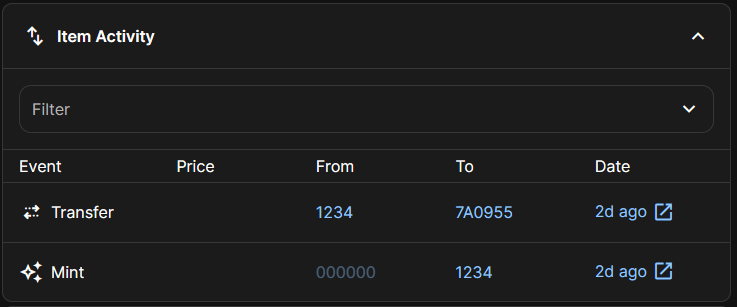
\includegraphics[width=1.1\textwidth]{OpenSea.PNG}
    \captionsetup{justification=centering}
    \caption{Tabella delle operazioni sull'NFT \cite{Ventidue}}
    \label{fig:OpenSea}
\end{figure}\newpage

\section{Come vendere il bene}
\label{sec:vendere}
Assumendo di avere ogni prodotto fisico con un QR code associato, fornirò ora un'idea per un possibile sistema finale per vendere un bene materiale, dalla vendita iniziale in negozio o online fino ad una possibile rivendita a terzi.\newline
Immaginiamo di avere un negozio fisico di una nota marca di prodotti di lusso e supponiamo che un cliente entri nel negozio con l'intenzione di acquistare una borsetta con un QR code associato.
\subsection{Primo acquisto}
Per mascherare i problemi dell'approccio 1:1 descritti nella \hyperref[sec:1to1]{Sezione 4.2}, è ragionevole creare gli NFT dinamicamente anziché a priori staticamente. In particolare, quando un cliente acquista una borsetta con QR code dal negozio fisico, l'NFT che protegge quella borsetta non sarà ancora stato creato. Perciò la prima volta che viene inquadrato il QR code verrà aperto un form. In questo sarà necessario inserire il proprio indirizzo pubblico insieme ad una OTP generata al momento dell'acquisto.\newline
Una volta svolta questa operazione, sarà eseguito automaticamente uno script che minterà l'NFT a nostro nome, che siamo stati incaricati di farlo, e successivamente lo trasferirà al cliente che lo ha acquistato, che sarà il primo proprietario effettivo.
\subsection{Controlli vari e acquisti successivi al primo}
Dopo la creazione e il trasferimento dell'NFT al primo proprietario, ogni qualvolta si inquadrerà il QR code verrà aperto OpenSea (come definito nella \hyperref[sec:presentare]{Sezione 6.2}) che permetterà di svolgere tutti i controlli del caso.\newline
Si noti che, in caso di acquisti successivi al primo, è fondamentale che il vecchio proprietario del bene materiale si occupi anche di trasferire l'NFT al nuovo proprietario, pena il non corretto funzionamento di tutto il sistema! Questa operazione può essere svolta, ad esempio, tramite un crypto wallet oppure andando a creare una pagina apposita che, dopo un'opportuna fase di autenticazione, esegua lo script della \hyperref[sec:trasferimento]{Sezione 5.6}.

\chapter{Conclusioni}
\noindent
In questo lavoro di tesi abbiamo terminato lo sviluppo di un sistema per garantire protezione ad un qualsiasi bene materiale.\newline
Dopo aver chiarito l'obiettivo, siamo partiti definendo una serie di concetti preliminari necessari ai fini del nostro progetto, tra cui alcuni strumenti utilizzati concretamente.\newline
Abbiamo proseguito scegliendo la blockchain su cui sviluppare effettivamente il sistema e, dopo aver compreso che avremmo utilizzato gli NFT, ci siamo occupati di selezionare l'approccio per la loro creazione che più si addiceva al nostro scopo.\newline
Successivamente ci siamo occupati di definire un metodo vero e proprio che permettesse di creare una serie di NFT sulla blockchain scelta e secondo l'approccio deciso. In particolare, siamo partiti da un documento di specifica contenente tutte le informazioni necessarie per il nostro obiettivo fino ad ottenere una serie di NFT di proprietà del cliente, uno per ogni oggetto da proteggere.\newline
Infine abbiamo visto alcuni spunti su come usare questi NFT in un possibile sistema concreto, concentrandoci su come associare l'NFT all'oggetto fisico, su come presentare l'NFT e su un possibile modo finale per vendere i beni e utilizzare la verifica tramite NFT per proteggerli.

\chapter{Ringraziamenti}
\noindent
Un sentito ringraziamento al Dott. Andrea Visconti per l'opportunità fornitami e per la passione e l'impegno dimostrato sia nelle lezioni del suo splendido corso di Crittografia I sia nel rapporto con i tirocinanti e con gli studenti tutti.\newline
Ringrazio poi la mia famiglia, in particolare i miei genitori Andrea e Roberta, per avermi supportato in questo lungo cammino di poco più di 3 anni, sostenendomi nei momenti di difficoltà e di sconforto e manifestando gioia e affetto per ogni scalino superato.\newline
Ringrazio infine tutti i miei amici e colleghi, in particolare Andrea e Nicholas, per aver portato spensieratezza nelle mie giornate, consigliandomi sempre saggiamente quando mi sono trovato di fronte a delle scelte importanti e aiutandomi a portare il peso di certe situazioni spiacevoli, permettendomi di terminare questo viaggio con il sorriso.

\begin{thebibliography}{unsrt}
    \bibitem{Uno}
    \textit{On the cryptography of Distributed Ledger Technology - 1. Hash Functions}\newline
    URL: \url{https://www.finriskalert.it/wp-content/uploads/visconti.pdf} (visitato il 14/03/2024)
    
    \bibitem{Due}
    \textit{Blockchain Merkle Trees}\newline
    URL: \url{https://www.geeksforgeeks.org/blockchain-merkle-trees/}\newline
    (visitato il 14/03/2024)

    \bibitem{Tre}
    \textit{Hash Pointers and Data Structures}. URL: \url{https://www.zhaohuabing.com/post/2018-05-12-cryptocurrency_week1_hash_pointer_and_data_structures/} (visitato il 14/03/2024)

    \bibitem{Quattro}
    \textit{What is blockchain?}\newline
    URL: \url{https://opensea.io/learn/blockchain/what-is-blockchain}\newline
    (visitato il 14/03/2024)

    \bibitem{Cinque}
    \textit{What is a smart contract?} URL: \url{https://opensea.io/learn/blockchain/what-is-a-smart-contract} (visitato il 15/03/2024)

    \bibitem{Sei}
    \textit{What is an NFT?}\newline
    URL: \url{https://opensea.io/learn/nft/what-are-nfts}\newline
    (visitato il 16/03/2024)

    \bibitem{Sette}
    Adeniyi E. A., Falola P. B., Maashi M. S., Aljebreen M., Bharany S.\newline
    \textit{Secure sensitive data sharing using RSA and ElGamal cryptographic algorithms with hash functions} (consultato il 17/03/2024)

    \bibitem{Otto}
    \textit{What is a crypto wallet?}\newline
    URL: \url{https://opensea.io/learn/web3/what-is-crypto-wallet}\newline
    (visitato il 17/03/2024)

    \bibitem{Nove}
    \textit{What is Etherscan?}\newline
    URL: \url{https://opensea.io/learn/blockchain/what-is-etherscan}\newline
    (visitato il 18/03/2024)

    \bibitem{Dieci}
    \textit{Etherscan}\newline
    URL: \url{https://etherscan.io/} (utilizzato il 07/10/2023)
    
    \bibitem{Undici}
    \textit{PolygonScan}\newline
    URL: \url{https://polygonscan.com/} (utilizzato il 15/10/2023)

    \bibitem{Dodici}
    \textit{What are EVM Compatible Blockchains? A Guide to the Ethereum Virtual Machine}. URL: \url{https://blog.thirdweb.com/evm-compatible-blockchains-and-ethereum-virtual-machine/} (visitato il 10/03/2024)

    \bibitem{Tredici}
    \textit{Update Report: Energy Efficiency and Carbon Footprint of the Polygon Blockchain}. URL: \url{https://carbon-ratings.com/dl/polygon-update-2022} (scaricato il 12/10/2023)

    \bibitem{Quattordici}
    \textit{Polygon for the Planet}. URL: \url{https://polygon.technology/sustainability} (visitato il 12/10/2023)

    \bibitem{Quindici}
    \textit{Certificato dell'opera "Between the Sky and Sea"}\newline
    URL: \url{https://www.pinterest.it/pin/344806915203383539/}\newline
    (visitato il 05/04/2024)

    \bibitem{Sedici}
    \textit{Dress from a Dream: Gold}. URL: \url{https://unxd.com/drops/dolce-gabbana-collezione-genesi/dress-from-a-dream-gold}\newline(visitato il 02/12/2023)

    \bibitem{Diciassette}
    \textit{Alchemy}\newline
    URL: \url{https://www.alchemy.com/} (utilizzato il 07/10/2023)
    
    \bibitem{Diciotto}
    \textit{MetaMask}\newline
    URL: \url{https://metamask.io/} (utilizzato il 04/10/2023)
    
    \bibitem{Diciannove}
    \textit{Polygon Mumbai Faucet}\newline
    URL: \url{https://www.alchemy.com/faucets/polygon-mumbai}\newline
    (utilizzato il 14/10/2023)

    \bibitem{Venti}
    \textit{PolygonScan Api Key Generator}\newline
    URL: \url{https://polygonscan.com/myapikey} (utilizzato il 09/12/2023)

    \bibitem{Ventuno}
    \textit{Pinata}\newline
    URL: \url{https://www.pinata.cloud/} (utilizzato il 09/10/2023)

    \bibitem{Ventidue}
    \textit{OpenSea}\newline
    URL: \url{https://opensea.io/learn} (utilizzato il 15/12/2023)
\end{thebibliography}

\end{document}